\section{Coverage del codice}

Sono stati svolti dei report di coverage del codice del pacchetto \texttt{quasylab.sibilla.core.network} per mezzo dei tre esempi di avvio del progetto. Tali report sono stati generati a partire dalla sottomissione di una simulazione da parte di un client e il conseguente processo di simulazione gestito dal server Master e dai server Slave, conclusasi senza la generazione di alcuna eccezione. Non sono quindi presenti all'interno del coverage le righe di codice inerenti alla gestione di tali eccezioni che si sarebbero potute sollevare a partire da una situazione di errore all'interno dell'infrastruttura.

\begin{figure}[H]
    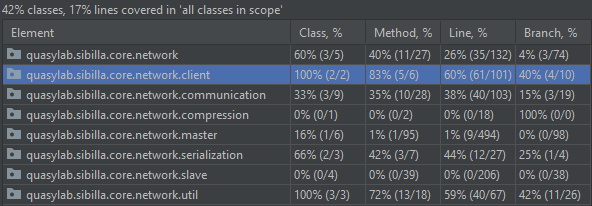
\includegraphics[width=\linewidth]{images/client_coverage.PNG}
    \captionsetup{justification=centering}
    \caption{Coverage del codice dell'esempio di avvio del Client}
  \end{figure}
  \begin{figure}[H]
    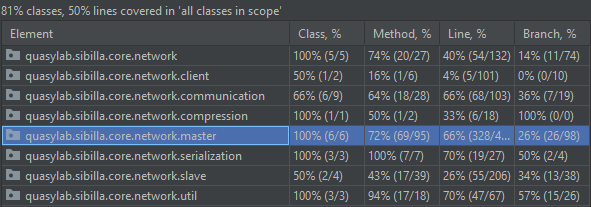
\includegraphics[width=\linewidth]{images/master_coverage.PNG}
    \captionsetup{justification=centering}
    \caption{Coverage del codice dell'esempio di avvio del server Master}
  \end{figure}
  \begin{figure}[H]
    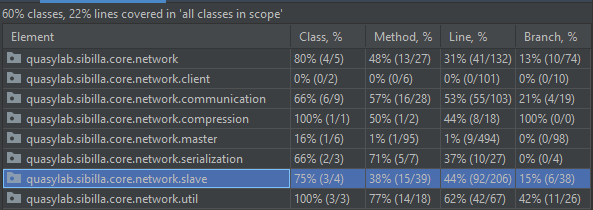
\includegraphics[width=\linewidth]{images/slave_coverage.PNG}
    \captionsetup{justification=centering}
    \caption{Coverage del codice dell'esempio di avvio del server Slave}
  \end{figure}